\subsection{Main Sequence of $5 \, {\rm \textbf{M}}_\odot$ and $9 \,{\rm \textbf{M}}_\odot$ Stars}
\begin{figure}[!ht]
    \centering
    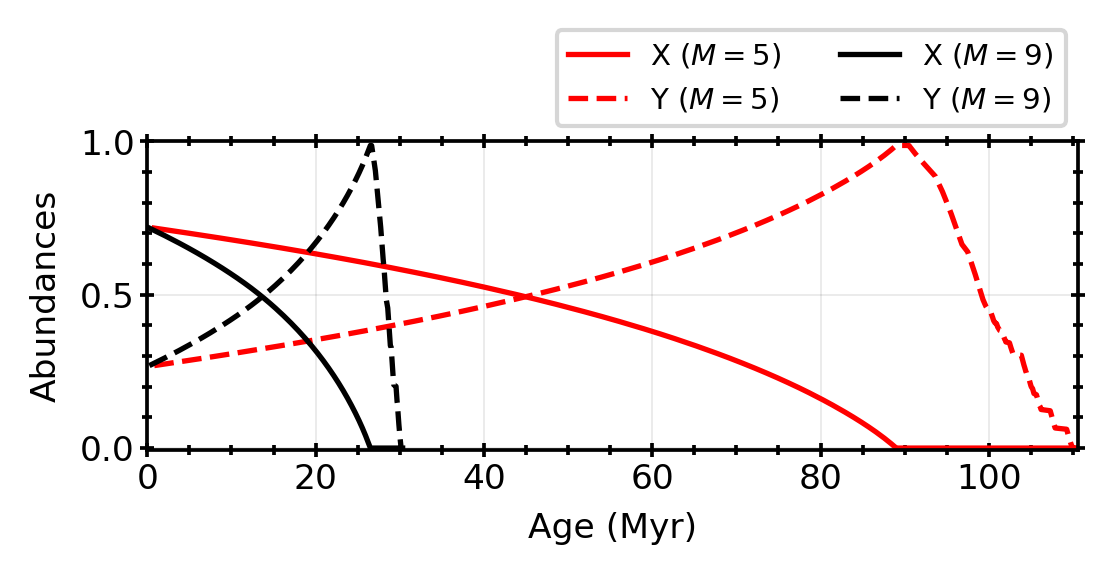
\includegraphics[width=1.0\columnwidth]{../figures/abundances.png}  % adjust the width as you like
    \caption{\small Abundances of H (solid line) and He (dashed line) over time for a $5 \, {\rm M}_\odot$ star (red) and a $9\, {\rm M}_\odot$ star.}
    \label{fig:abundances}
\end{figure}
We start by looking at the abundances of Hydrogen, $X$ and Helium, $Y$, for a $5 \, {\rm M}_\odot$ star and a $9 \, {\rm M}_\odot$ star. Results are represented in Figure \ref{fig:abundances}. We see how $X$ decreases significantly faster for $ 9 \,{\rm M}_\odot$ than for $5 \,{\rm M}_\odot$.

The H abundance allows us to define the MS lifetime of a star, $\tau_{\rm MS}$, as the time the star is steadily burning H in its core, with the MS ending with H core-exhaustion. For the stellar models we are working with, $\tau_{\rm MS}$ can be defined as
\begin{align}
    \tau_{\rm MS} & = t_n - t_0 \ , \ \ {\rm where}                                                              \notag              \\
    n             & = {\rm min}\{i\in \mathbb{N} \ | \  1 \leq i \leq N \ {\rm and} \ X_i < \varepsilon\} \ . \label{eq:MS_lifetime}
\end{align}
for a given cutoff H exhaustion abundance, $\varepsilon$. That is, it is defined as the time it takes for the H abundance,
$X$, to drop below $\varepsilon$. Choosing $\epsilon = 10^{-3}$ we find that $\tau_{\rm MS} = 8.82 \times 10^6$ yr for a $5 \, {\rm M}_\odot$ star and $\tau_{\rm MS} = 2.63 \times 10^6$ yr for a $9 \, {\rm M}_\odot$ star. The MS lifetime is shorter for the more massive star, which is in accordance with the H-burning rates observed in Figure \ref{fig:abundances}. This result is expected as more massive stars have higher H-burning rates, due to the higher temperatures and pressures in their cores that allow for the CNO fusion cycle to take place. Low mass stars, on the other hand, burn H through the $p\text{--}p$ chain reaction, which is less efficient than the CNO cycle and leads to longer MS lifetimes.
% \onecolumn
% \twocolumn


\subsection{Hertzprung--Russell Diagram}

\begin{figure}[!ht]
    \centering
    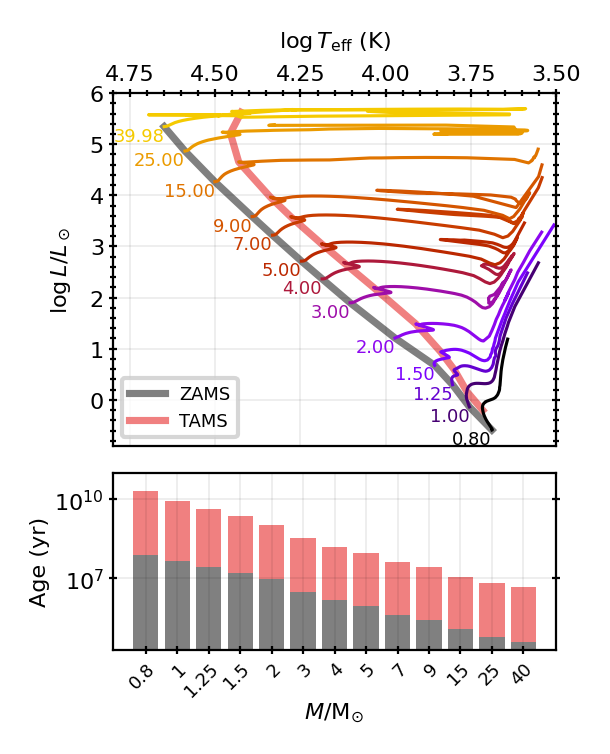
\includegraphics[width=1.0\columnwidth]{../figures/HR_plot.png}  % adjust the width as you like
    \caption{\small (Top) HR diagram showcasing stellar evolution tracks for stellar models with different masses. The grey line represents the ZAMS for all models. The pale-red line represents the TAMS for all models. Numbers represent the mass of the star in units of ${\rm M}_\odot$. (Bottom) Values of the ZAMS (grey) and TAMS (pale-red).}
    \label{fig:HR_plot}
\end{figure}



\begin{table}[!ht]
    \centering
    \caption{\small Values of the ZAMS and TAMS for models with different stellar masses.}
    \begin{tabular}{|c|l|l|}
        \hline
        Mass  & ZAMS                 & TAMS                  \\ \hline
        0.80  & $7.48 \times 10^{7}$ & $2.16 \times 10^{10}$ \\ \hline
        1.00  & $4.49 \times 10^{7}$ & $8.53 \times 10^{9}$  \\  \hline
        1.25  & $2.74 \times 10^{7}$ & $4.23 \times 10^{9}$  \\ \hline
        1.50  & $1.60 \times 10^{7}$ & $2.24 \times 10^{9}$  \\ \hline
        2.00  & $9.15 \times 10^{6}$ & $1.02 \times 10^{9}$  \\ \hline
        3.00  & $2.86 \times 10^{6}$ & $3.23 \times 10^{8}$  \\ \hline
        4.00  & $1.43 \times 10^{6}$ & $1.53 \times 10^{8}$  \\ \hline
        5.00  & $8.33 \times 10^{5}$ & $8.90 \times 10^{7}$  \\ \hline
        7.00  & $4.02 \times 10^{5}$ & $4.21 \times 10^{7}$  \\ \hline
        9.00  & $2.49 \times 10^{5}$ & $2.65 \times 10^{7}$  \\ \hline
        15.00 & $1.18 \times 10^{5}$ & $1.11 \times 10^{7}$  \\ \hline
        25.00 & $5.97 \times 10^{4}$ & $6.36 \times 10^{6}$  \\ \hline
        39.98 & $3.64 \times 10^{4}$ & $4.47 \times 10^{6}$  \\ \hline
    \end{tabular}
    \label{tab:ages}
\end{table}

\newpage

Stellar evolution tracks for different stellar masses are represented in Figure \ref{fig:HR_plot} (Top). The values of the Zero-Age-MS (MS) and Terminal-Age-MS (TAMS) are represented in \ref{fig:HR_plot} (Bottom), with values in Table \ref{tab:ages}. Integration of stellar models starts at the ZAMS, thus ${\rm ZAMS} = t_1$ for all models. The TAMS is defined as the time at which the star has exhausted all of its H in the core, thus ${\rm TAMS} = t_n$ for all models, with $n$ being the index defined in Eq. \eqref{eq:MS_lifetime} for an H-exhaustion cutoff $\varepsilon=10^{-3}$.

High stellar mass stars have significantly shorter MS lifetimes than low stellar mass stars. The MS lifetime for the the  $0.8 \, {\rm M}_\odot$ star model is $21.46$ Gyr, while the MS lifetime for the $\sim 40 \, {\rm M}_\odot$ star is $4.44$ Myr, more than 4 orders of magnitude shorter. The main reason is that high mass stars have higher core concentration and temperature which leads to more efficient nuclear reactions. This is reflected in the fact that the nuclear reaction rate is given by
\begin{equation}
    q_{\rm nuc} \propto \rho T^n \ ,
\end{equation}
with $n$ depending on the nuclear reaction, which in itself depends also on $T$. For the $p\text{--}p$ chain, $n=4$, while for the CNO cycle, $n=16$.

%the fact that high mass stars have higher H-burning rates, as they have higher temperatures and pressures in their cores that allow for the CNO fusion cycle to take place. Low mass stars, on the other hand, burn H through the $p\text{--}p$ chain reaction, which is less efficient than the CNO cycle and leads to longer MS lifetimes.

% \onecolumn
% \twocolumn

\subsection{Homology Relations}

We now analyze the $\log L \text{--} \log M$, $\log T_c \text{--} \log M$ and $\log \rho_c \text{--} \log M$ relations for the stellar models at the ZAMS. We do so for stellar models of mass: 0.8, 1.0, 1.25, 1.5, 2.0, 3.0, 4.0, 5.0, 7.0, 9.0, 15.0, 25.0 and 39.98 ${\rm M}_\odot$. Let us define
\begin{align}
    \alpha & \equiv \frac{\log L}{\log M} \ , \label{eq:alpha}      \\
    \beta  & \equiv \frac{\log \rho_c}{\log M} \ ,  \label{eq:beta} \\
    \gamma & \equiv \frac{\log T_c}{\log M} \ . \label{eq:gamma}
\end{align}
to be the slopes of the $\log L \text{--} \log M$, $\log T_c \text{--} \log M$ and $\log \rho_c \text{--} \log M$ relations for the stellar models at the ZAMS. We compute each slope ($\alpha$, $\beta$ and $\gamma$) for sets of low, mid and high mass stars. The (rough) criteria for mass classification is as follows:
\begin{itemize}
    \item \textbf{Low mass}: $0.35 \, {\rm M}_\odot < M < 2 \, {\rm M}_\odot$. Stars that burn H through the $p\text{--}p$ chain reaction and are governed by a Kramers opacity law.
    \item \textbf{Mid mass}: $ 2 \, {\rm M}_\odot \leq M < 10 \, {\rm M}_\odot$. Stars that burn H through the CNO cycle and are governed by a Kramers opacity law.
    \item \textbf{High mass}: $M \geq 10 \, {\rm M}_\odot$. Stars that burn H through the CNO cycle and are governed by a constant opacity coming from electron scattering.
\end{itemize}
These slopes are represented in Figure \ref{fig:regressions} for the different mass ranges of the stellar models. It is our goal now to compare these slopes with the slopes predicted by homology relations found in the literature for MS stars. The slopes found with homology relations are dependent on the mass ranges, as these are affected by the opacity law governing the star and its nuclear burning rate, which is different for the $p\text{--}p$ chain and the CNO cycle. Finding the slopes through homology relations is rather cumbersome, and an outline of their derivation is included in Appendix A. For stars governed by a Kramers opacity law  (low and mid mass stars), we find the following homology relations\footnote{Homology relations for the density are found for the mean density of the star, which we assume to be representative of the density at the core, $\rho_c$.}:
\begin{align}
    \alpha & = \frac{10n +31}{5 + 2n}                                                              \\
    \beta  & =  \frac{2\left(n-3 \right)\left(2n+11 \right)}{\left(n+3 \right)\left(2n+ 5 \right)} \\
    \gamma & = \frac{-8n - 44}{\left(n+3 \right)\left(2n+ 5 \right)}
\end{align}
where $n$ refers to the exponent of the temperature in the the nuclear burning rate equation $q_{\rm nuc} \propto \rho T^n $, with $n=4$ for the $p\text{--}p$ chain (low mass) and $n=16$ for the CNO cycle (mid mass). On the other hand, for stars governed by a constant opacity (high mass), we find:
\begin{align}
    \alpha & = 3                 \\
    \beta  & =  \frac{6-2n}{3+n} \\
    \gamma & =  \frac{-4}{n+3}
\end{align}
where we always set $n=16$ as high mass stars burn H through the CNO cycle.

The comparison between values found from the stellar model data and homology relations is represented in Table \ref{tab:regression}. We find that the slopes for the $\log L \text{--} \log M$ relation are in somewhat good agreement with the homology relations for all mass ranges, with the highest relative error being $0.297$ for mid mass stars.
The slopes for the $\log \rho_c \text{--} \log M$ found from the homology relations fail for low and high mass stars. We believe this is due to the rather wild assumption of associating the density of the star with the density in the core when deriving these relations (see footnote).
Finally, the slopes for the $\log T_c \text{--} \log M$ relation are also in somewhat good agreement, with the highest deviation occurring for high mass stars (0.325 relative error).


%The slopes for the $\log \rho_c \text{--} \log M$ relation are in good agreement for low and mid mass stars, but not for high mass stars. Finally, the slopes for the $\log T_c \text{--} \log M$ relation are in good agreement for low mass stars, but not for mid and high mass stars. The slopes for the $\log T_c \text{--} \log M$ relation are the least accurate, which is expected as the temperature in the core is not constant throughout the simulation, and thus the slope is not constant either. The slopes for the $\log \rho_c \text{--} \log M$ relation are more accurate, as the density in the core is more constant than the temperature. Finally, the slopes for the $\log L \text{--} \log M$ relation are the most accurate, as the luminosity is the most constant of the three magnitudes. 

\begin{table}[h!]
    \centering
    \captionsetup[table]{width=0.8\textwidth}
    \caption{\small Slopes of the $\log L \text{--} \log M$ ($\alpha$), $\log \rho_c \text{--} \log M$ ($\beta$) and $\log T_c  \text{--} \log M$ ($\gamma$) relations for low, mid and high mass stars (see main text for mass classification criteria). Slopes are computed from model data and homology relations, and the relative error is included in the table. Model data is represented in Figure \ref{fig:regressions}.}
    \begin{tabular}{|c|c|c|c|}
        \cline{2-4}
        \multicolumn{1}{c|}{} & Model Data & Hom. Rels. & Rel. Error \\ \cline{2-4}\noalign{\vspace{0.2em}}\hline
        $\alpha_{\rm low}$    & $4.61$     & $5.46$     & $0.156$    \\ \hline
        $\beta_{\rm low}$     & $0.144$    & $0.769 $   & $0.813$    \\ \hline
        $\gamma_{\rm low}$    & $0.727 $   & $0.923 $   & $0.212$    \\ \hline\hline
        $\alpha_{\rm mid}$    & $3.63$     & $5.16$     & $0.297$    \\ \hline
        $\beta_{\rm mid}$     & $-1.20$    & $-1.03$    & $-0.167$   \\ \hline
        $\gamma_{\rm mid}$    & $0.264$    & $0.324$    & $0.186$    \\ \hline\hline
        $\alpha_{\rm high}$   & $2.53   $  & $3.00$     & $0.156$    \\ \hline
        $\beta_{\rm high}$    & $- 0.805$  & $-1.37$    & $0.412 $   \\ \hline
        $\gamma_{\rm high}$   & $0.142$    & $0.211$    & $ 0.325$   \\ \hline
    \end{tabular}
    \label{tab:regression}
\end{table}

% \onecolumn

\begin{figure*}[h]
    \centering
    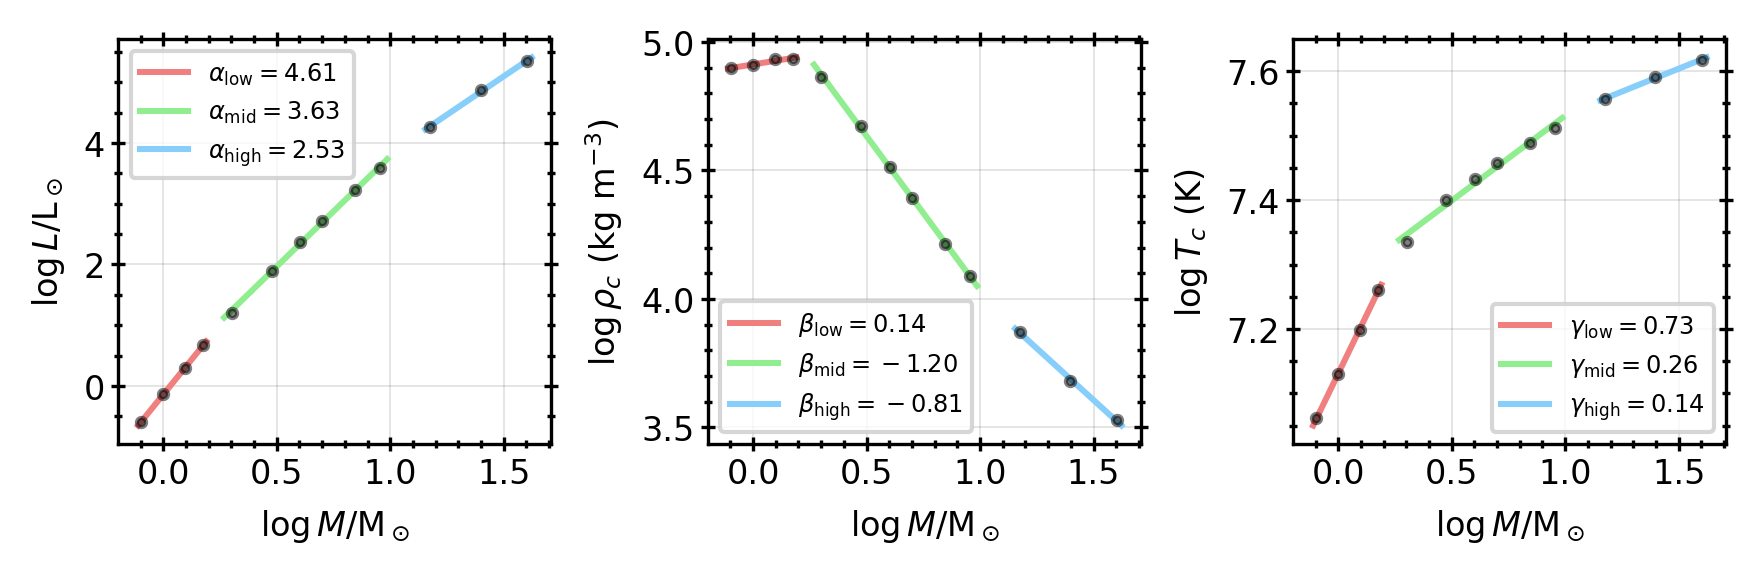
\includegraphics[width=1.0\textwidth]{../figures/regressions.png}  % adjust the width as you like
    \caption{\small Slopes of the $\log L \text{--} \log M$ ($\alpha$), $\log \rho_c \text{--} \log M$ ($\beta$) and $\log T_c  \text{--} \log M$ ($\gamma$) relations for low, mid and high mass stars (see main text for mass classification criteria). In solar mass units, low mass stars are 0.8, 1.0, 1.25 and 1.5; mid mass stars are 2.0, 3.0, 4.0, 5.0, 7.0 and 8.0; and high mass stars are 14.0, 25.0 and 39.98.}
    \label{fig:regressions}
\end{figure*}




\onecolumn
\twocolumn

\subsection{The $\log T_c \text{--} \log \rho_c$ Plane}


\begin{figure}[!ht]
    \centering
    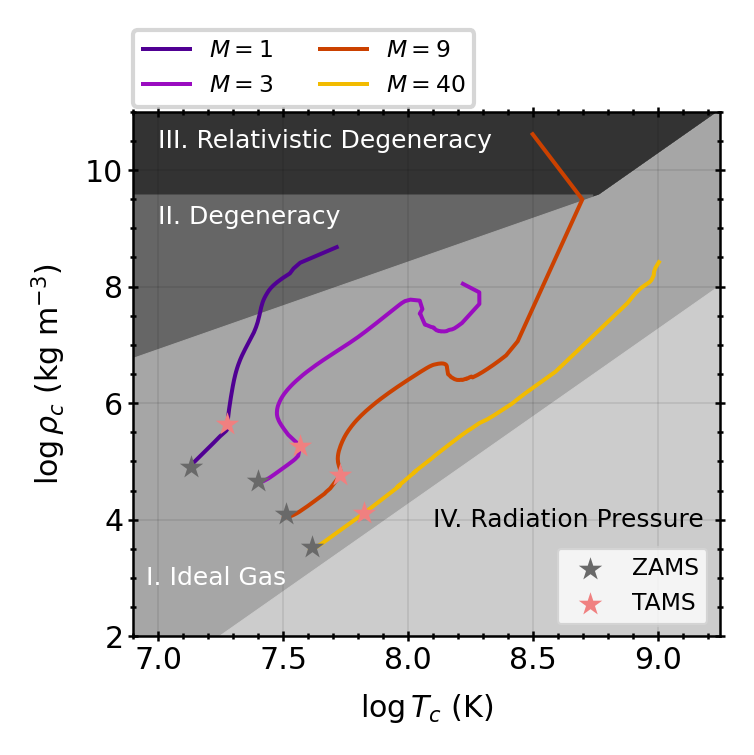
\includegraphics[width=1.0\columnwidth]{../figures/t_rho_tracks.png}  % adjust the width as you like
    \caption{\small Stellar evolution tracks in the $\log T_c \text{--} \log \rho_c$ plane for stellar models with masses 1.0, 3.0, 9.0 and 40.0 ${\rm M}_\odot$. The position of the ZAMS and the TAMS are marked with a pale-red and grey star respectively. The grey filling represents the domains where the star's core equation of state is governed by radiation pressure, the ideal gas law (for ions and electrons), electron degeneracy pressure, and relativistic electron degeneracy pressure.}
    \label{fig:tc_rhoc}
\end{figure}

Representing a star in the $\log T_c \text{--} \log \rho_c$ plane allows us to identify the equation of state governing the core of the star. The four regimes are
\begin{itemize}
    \item \textbf{Clasical Ideal Gas Regime}: The equation of state for the ion and electron gas is
          \begin{equation}
              P_{\rm id} = \frac{\mathcal{R}}{\mu} \rho_c T_c
          \end{equation}
          where $\mathcal{R} \equiv k_{\rm B} / m_{\rm H} = 8314 \, {\rm J}{\rm K}^{-1} {\rm kg}^{-1}$  is the gas constant and $\mu$ is the mean molecular weight ot the ions and electrons, which we set to $0.61$.
    \item \textbf{Degenerate Electron Gas Regime}: The equation of state is
          \begin{equation}
              P_{\rm e-d} = K_1 \rho_c^{5/3}
          \end{equation}
          where
          \[
              K_1 = \left( \frac{3}{\pi} \right)^{\frac{2}{3}} \frac{h^2}{m_e \left(2 m_H \right)^{5/3}}
          \]
    \item \textbf{Relativistic Electron Degeneracy Regime}: The equation of state is
          \begin{equation}
              P_{\rm e-rd} = K_2 \rho_c^{4/3}
          \end{equation}
          where
          \[
              K_2 = \left( \frac{3}{\pi} \right)^{\frac{1}{3}} \frac{h c}{8 \left(2 m_H\right)^{4/3}}
          \]
    \item \textbf{Radiation Pressure Regime}: The equation of state is
          \begin{equation}
              P_{\rm rad} = \frac{1}{3}aT_c^4
          \end{equation}
          where
          \[
              a = \frac{8 \pi^5 k_\text{B}^4}{15 c^3 h^3}
          \]
\end{itemize}

By equating the different equations of state we can find the boundaries between the different regimes in the $\log T_c \text{--} \log \rho_c$ plane. These boundaries are represented in Figure \ref{fig:tc_rhoc} alongside the stellar evolution tracks for stellar models with masses 1.0, 3.0, 9.0 and 40.0 ${\rm M}_\odot$. We observe that only the 1 ${\rm M}_\odot$ star reaches electron degeneracy, while the 9 ${\rm M}_\odot$ directly reaches relativistic electron degeneracy.


\subsection{Analysis of a 4$\,$M$_\odot$ star}

We present now a thorough analysis of the evolution of the 4$\,$M$_\odot$ stellar model. Relevant stellar magnitudes are represented in Figure \ref{fig:ex4}. The --coarse-grained-- phases of stellar evolution are:
\begin{itemize}
    \item \textbf{Main Sequence (MS)} (A$\rightarrow$B): The star steadily burns H in its core through the CNO cycle. Instead of defining the MS lifetime as the time it takes for the H abundance to drop below an insignificant H-exhaustion cutoff $\varepsilon=10^{-3}$ (as done in Section 2.1), we set $\varepsilon=0.03$. This way we differentiate the MS from the Hook (B$\rightarrow$C) (see next bullet point). We find that the star is in its MS from 1.43 to 151.28 Myr, corresponding to a MS lifetime of $149.85$ Myr. The nucleus contracts and heats up, as $\rho_c$ and $T_c$ steadily increase. $L$ increases and $T_eff$ decreases. The radius \footnote{Not provided in the model data. It is computed using Stefan-Boltzmann Law: $L=4\pi R^2 T_{\rm eff}^4$.} $R$ increases slowly from $2.15$ to $4.69 \, {\rm R}_\odot$.
    \item \textbf{Hook} (B$\rightarrow$C): Last stage of H burning as the star contracts in a Kelvin-Helmontz timescale. $R$ decreases from $4.69$ to $4.16 \, {\rm R}_\odot$ with its consequent increase in $T_{\rm eff}$, which creates a hook-like bend in the HR diagram. $T_c$ and $\rho_c$ increase proceed. The star is in this phase from 151.28 to 153.44 Myr, lasting $2.61$ Myr.
    \item \textbf{Hertzprung Gap (HG)} (C$\rightarrow$D): Hydrogen has exhausted in the core and shell H burning proceeds. The core stars collapsing and the envelope of the star expands, with $R$ increasing from $4.16$ to $18.63 \, {\rm R}_\odot$. As core burning has stopped, and due to out-of-equilibrium processes $L$ decreases. We identify the end of this phase when $L$ starts to increase again. The star is in this phase from 153.44 to 156.22 Myr, lasting $2.78$ Myr.
    \item \textbf{Red Giant Branch (RGB)} (D$\rightarrow$E): The core keeps contracting and heating up. $R$ continues to increase rapidly from $18.63$ to $50.74 \, {\rm R}_\odot$ as the star's envelope expands. As $T_{\rm eff}$ is roughly constant, $L$ increases with $R$. This phase ends when the core has heat up enough to burn He. The star is in this phase from 156.22 to 156.94 Myr, lasting $0.72$ Myr.
    \item  \textbf{Blue Loop (BL)} (E$\rightarrow$F): The core starts burning He. C and N abundances increase. It is a complex phase. TThe star performs a loop towards the blue region of the HR diagram and ends up in roughly the same place it started from. $R$ decreases from 50.74 to 31.47 ${\rm R}_\odot$. This phase ends when the core runs out of He. The star is in this phase from 156.94 to 194.48 Myr, lasting $37.54$ Myr.
    \item  \textbf{Asymptotic Giant Branch (AGB)} (F onwards): He burning stops. The core contracts and the envelope rapidly expands. $R$ and $L$ rapidly increase. The simulation run ends early in this phase, at 195.53 Myr age.
\end{itemize}

The radius $R$ rapidly increases in two phases: during the HG$+$RGB and during the AGB. In both phases the core contracts and the envelope expands due to the mirror effect. In the HG$+$RGB the core contracts due to the exhaustion of H, and in the AGB the core contracts due to the exhaustion of He.

The model run ends early in the AGB phase. During this phase and onwards, the star has exhausted H and He in its core and burns these elements in shells surrounding a core mainly composed of C and O. The star begins a period of pulsations with recurrent surges in He burning and material being expelled from the outer layers of the star. A planetary nebulae forms. As the planetary nebulae disperses, the core of the star contracts and becomes a white dwarf.

\begin{figure*}[!ht]
    \centering
    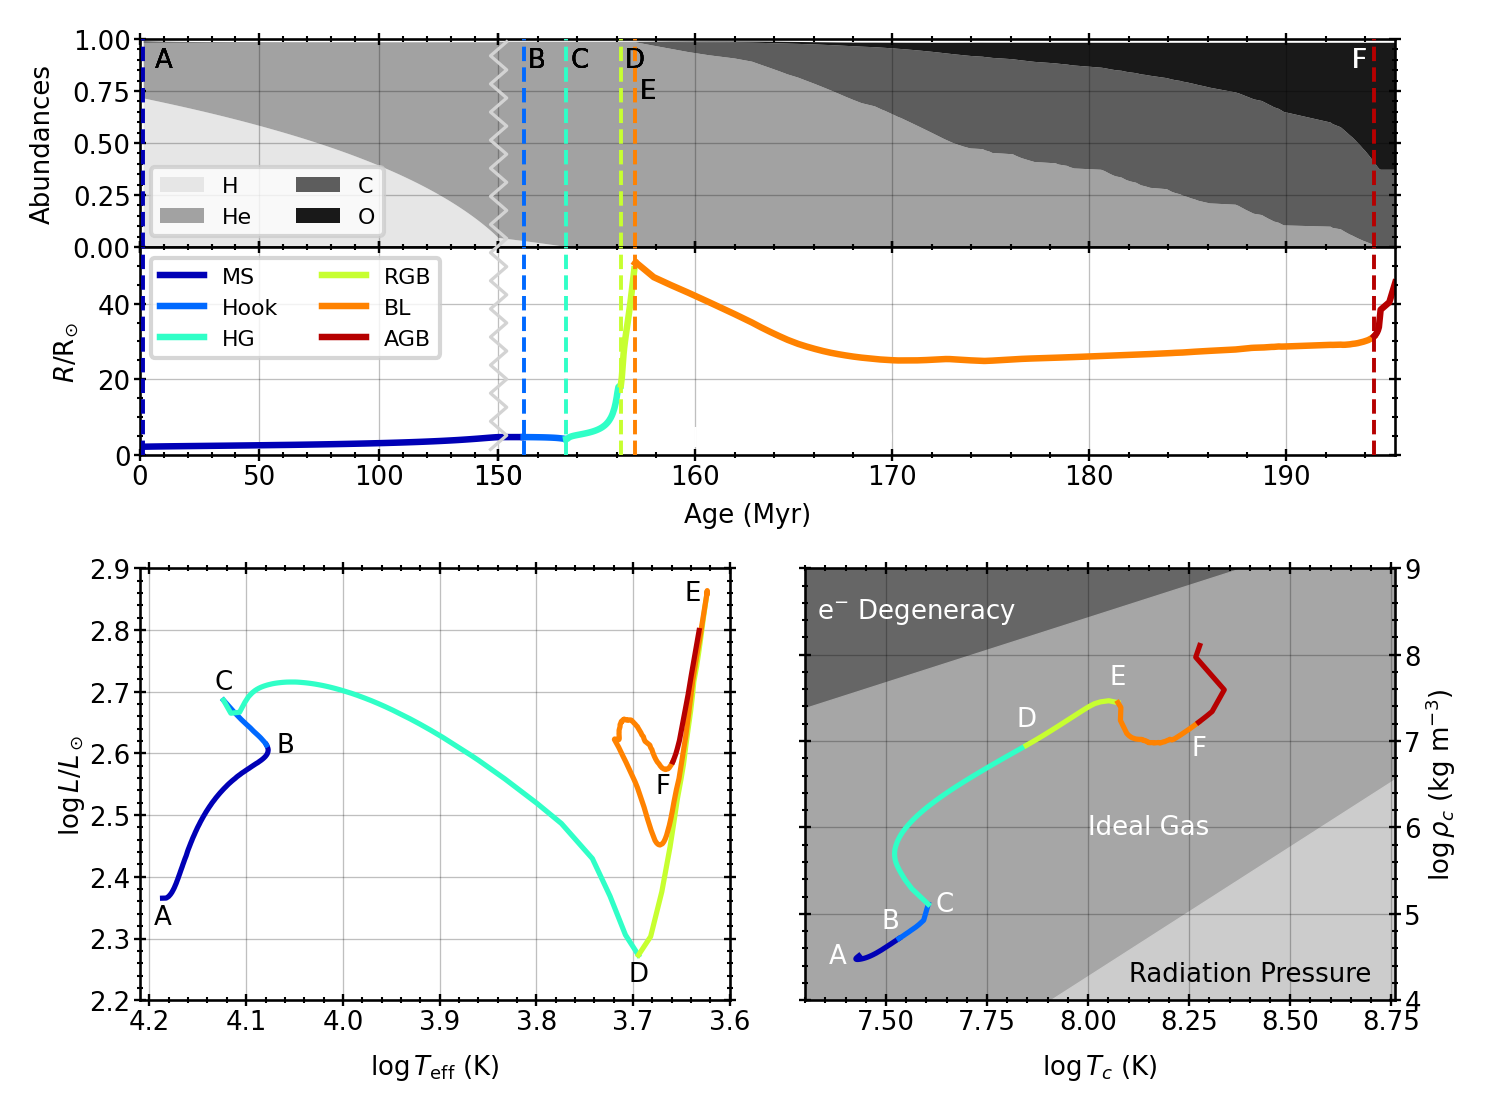
\includegraphics[width=1.0\textwidth]{../figures/ex4.png}  % adjust the width as you like
    \caption{\small Evolution of a $4 \, {\rm M}_\odot$ star. Different phases of stellar evolution are depicted with letters and colors: Main Sequence (MS) in dark blue, A$\rightarrow$B; Hook in light blue, B$\rightarrow$C; Hertzprung Gap (HG) in cyan, C$\rightarrow$D; Red Giant Branch (RGB) in yellow, D$\rightarrow$E; Blue Loop (BL) in orange, E$\rightarrow$F; and Asymptotic Giant Branch (AGB) in red, F onwards. (Top) Time series for abundances of H, He, C and O. (Middle) Time series for teh radius $R$. (Bottom-Left) Evolutionary track in the HR diagram. (Bottom-Right) Evolutionary track in the $\log T_c \text{--} \log \rho_c$ plane, with greyed filling indicating the equation of state regimes of the core.}
    \label{fig:ex4}
\end{figure*}
